\section{Resolution, rankings and reporting freedom}\label{sec:results}

\subsection{No rule leads across collections}\label{sec:coll}

Appendix Table~\ref{tab:collections2} gives the accuracy of every rule on every collection (Figure~\ref{fig:collections} in the appendix).



\begin{figure}[t]
\centering
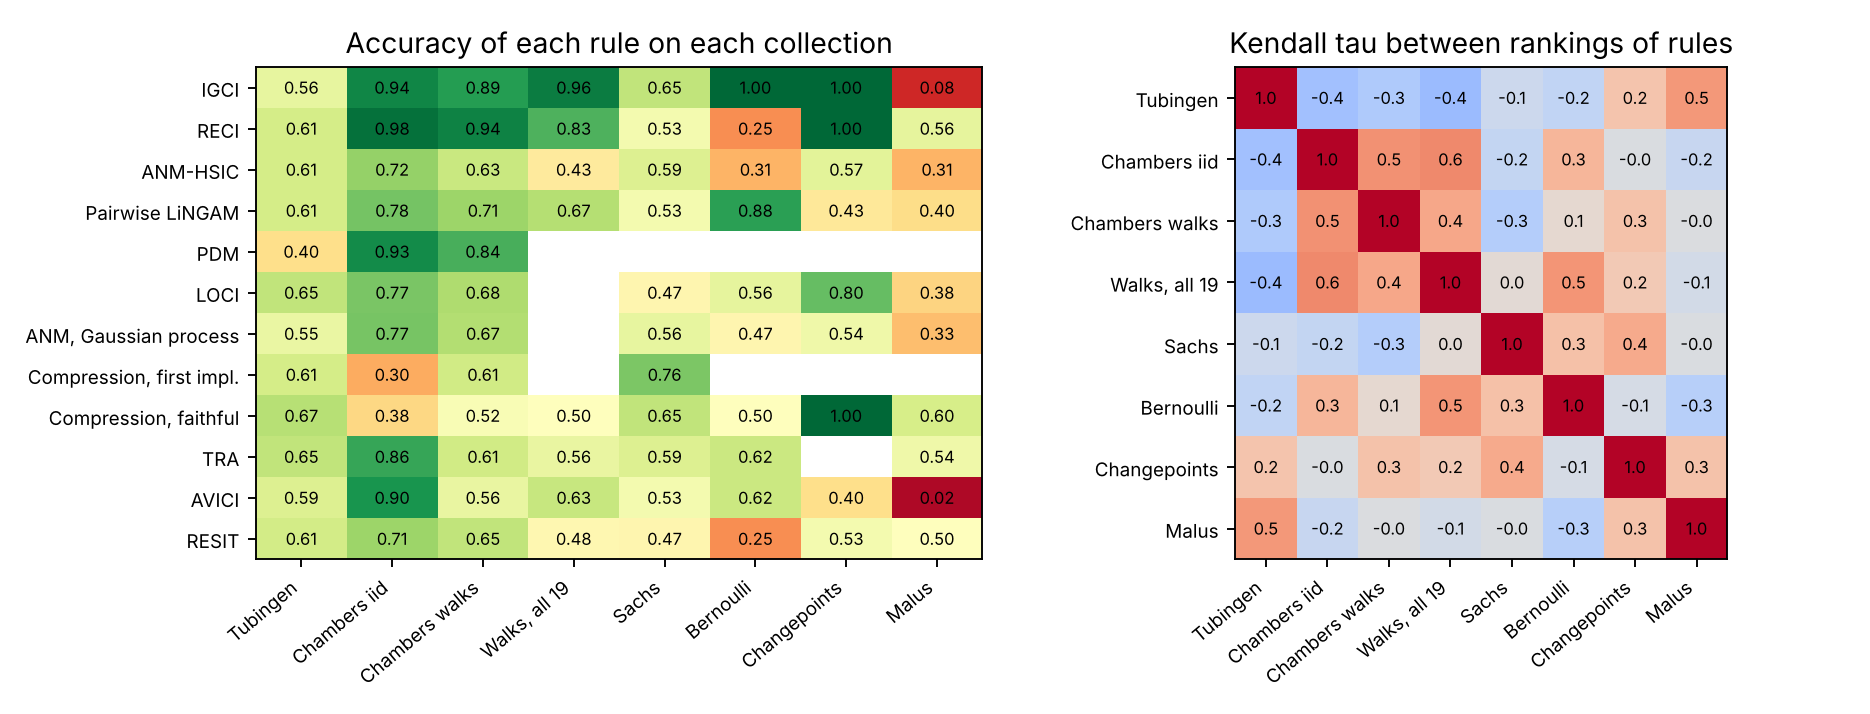
\includegraphics[width=\linewidth]{figs/collections.png}
\caption{Left: accuracy of every rule on every collection (all rules on raw arrays; T\"ubingen dequantised). Right: Kendall rank correlation between the orderings of the rules on two collections (rules run on both; at least five); none is distinguishable from zero after correction.}
\label{fig:collections}
\end{figure}

\paragraph{(1) The leader changes.} Round255 compression leads T\"ubingen ($66.7\%$; LOCI and TRA at $64.7$ and $64.6\%$) and Malus ($60.4\%$), RECI the two chamber collections with independent or random-walk actuators ($97.9\%$ and $94.3\%$), IGCI the $19$ untouched walk recordings ($95.7\%$; RECI $82.9\%$) and the Bernoulli collection ($100\%$), floor256 compression the $17$ Sachs pairs ($76.5\%$; round255 $64.7\%$), and IGCI, RECI and round255 compression tie on the changepoint pairs ($100\%$). Four of the twelve rules lead at least one collection. IGCI is above $70\%$ on five collections and at $8.3\%$ on Malus and $55.9\%$ on T\"ubingen; RECI is above $70\%$ on four; pairwise LiNGAM on three; no other rule on more than two. The additive-noise rules lead nowhere: ANM-HSIC is at $43.4\%$ on the $19$ walk recordings, RESIT at $47.5\%$.

\paragraph{(2) Rules that agree on one collection disagree on the next.} In our implementation IGCI orients the Bernoulli and changepoint pairs correctly in every case and the Malus pairs wrongly in $44$ of $48$. RECI is at $25\%$ on the Bernoulli pairs. The pretrained AVICI model, run on two-variable inputs, is at $90.4\%$ on the i.i.d.\ chambers and $2.1\%$ on Malus. Round255 compression is at $100\%$ on the changepoint pairs, $60.4\%$ on Malus and $38.3\%$ on the i.i.d.\ chambers. With the recordings as clusters, sign-flip tests give IGCI above RECI on the $19$ walk recordings ($p=0.019$) and RECI above ANM-HSIC, AVICI and pairwise LiNGAM ($p<0.001$); on the i.i.d.\ chambers ($47$ edges as clusters) RECI is above ANM-HSIC ($p<0.001$) and IGCI above ANM-HSIC ($p=0.012$), while IGCI and RECI are not separated ($p=0.63$); with five recordings the smallest attainable $p$ is $0.0625$.

\paragraph{(3) Rankings do not clearly transfer.} Kendall's $\tau$ between the ordering of the rules on T\"ubingen and on the i.i.d.\ chambers is $-0.38$, on the walks $-0.30$ ($-0.42$ for all $19$ recordings), on Sachs $-0.12$, on Bernoulli $-0.19$; it is $+0.24$ against the changepoints and $+0.51$ against Malus. Of the $28$ correlations one has a raw permutation $p<0.05$ (i.i.d.\ against walks, $0.02$) and none survives a Holm correction (smallest adjusted $p=0.49$): the T\"ubingen accuracies span twelve points with intervals of $\pm0.10$, so the ordering of the rules on that collection is mostly noise, and the data support no statement of agreement or disagreement between collections at the level of rank correlations.

\paragraph{Cautions.} The i.i.d., walk, Bernoulli, changepoint and Malus collections are best read as case studies of regimes of two devices, not as samples of mechanisms: they have $47$, $\le65$, $8$, $7$ and $4$ distinct edges, the cause is an experimenter-set actuator and the effect a sensor. Cluster-bootstrap intervals (Appendix Table~\ref{tab:collections_ci}) are degenerate with fewer than nine clusters. The T\"ubingen arrays are dequantised, a convention that matters (on raw arrays IGCI is at $63.8\%$ on average over the configurations of Section~\ref{sec:protocol_multiverse} against $52.4\%$ dequantised). The leads of round255 compression on T\"ubingen and Malus rest on one pair over LOCI ($p=0.88$) and on three points with four clusters.


\subsection{Sampling noise}\label{sec:noise}

Appendix Table~\ref{tab:multi} gives the accuracies on T\"ubingen with exact Clopper--Pearson intervals. The half-width is about $0.10$ for every rule, and the intervals treat the pairs as independent, which they are not exactly (the official weights downweight groups of similar pairs; unweighted accuracy is used). All rules are evaluated on the same pairs, so the right comparison between two rules is the exact McNemar test on the pairs on which exactly one is correct; exact ties (a score of zero) and pairs on which a rule returned no value (TRA, $20$ pairs) are left out of the discordant counts, so TRA is compared on a different sample.

\begin{figure}[t]
\centering
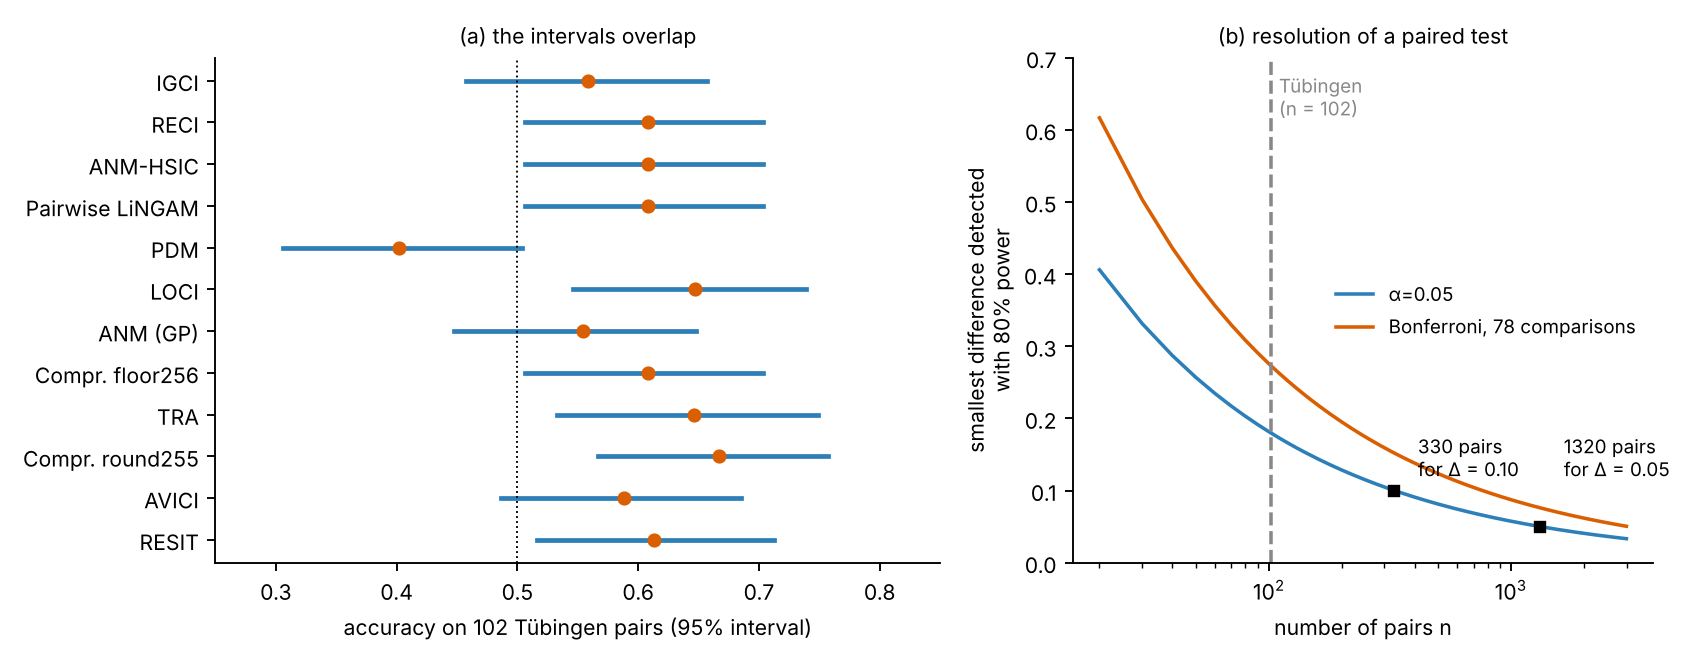
\includegraphics[width=\linewidth]{figs/fig3_resolution.png}
\caption{(a) Accuracy of the twelve rules on the $102$ T\"ubingen pairs with exact $95\%$ intervals. (b) Analytic smallest difference in accuracy detected with $80\%$ power by a paired test, as a function of the number of pairs, for a discordance rate of $0.42$.}
\label{fig:resolution}
\end{figure}

\paragraph{Two families of comparisons.} The first family has the twelve rules of Appendix Table~\ref{tab:collections2} plus the floor256 compression with raw rows: $78$ comparisons. Twelve have a raw $p<0.05$ and two survive a Holm correction (smallest adjusted $p=0.015$); both involve the learned classifier PDM, which is below chance (PDM against round255 compression and against LOCI; all $12$ raw-significant comparisons involve PDM), so they say nothing about the other rules. The second family fixes the ten rules that are not degenerate and not duplicated (IGCI, RECI, ANM-HSIC, pairwise LiNGAM, LOCI, ANM-GP, round255 compression, TRA, AVICI, RESIT; without PDM and without the other compression variants): $45$ comparisons, \emph{none} with a raw $p<0.05$ (smallest raw $p=0.11$, ANM-GP against RESIT). The result is the same on the common set of the $82$ pairs on which all ten rules return a value (exact ties counted as half in both cells of the discordance table): none of the $45$ comparisons has a raw $p<0.05$ (smallest $0.078$, ANM-GP against TRA). PDM's accuracy of $40.2\%$ is not a sign error: the same classifier and sign convention give $93\%$ and $84\%$ on the two chamber collections, so its failure on T\"ubingen is a failure to transfer from the simulator, which we did not diagnose further. For the best rule, round255 compression ($66.7\%$), the tests against RECI, LOCI, IGCI, ANM-GP and AVICI have $p=0.39$, $0.88$, $0.14$, $0.20$ and $0.35$ (discordant pairs $20$/$14$, $23$/$21$, $29$/$18$, $24$/$15$, $32$/$24$).

\paragraph{Detectable difference.} With the observed rate of discordant pairs ($42\%$, computed on pairs where both rules have a value and neither ties; averaged over the $78$ comparisons), a simulated paired comparison on $102$ pairs reaches $80\%$ power for a difference in accuracy of $0.19$ at level $0.05$ and of $0.27$ with a Bonferroni correction over the $78$ comparisons. The simulation draws the number of discordant pairs from the observed rate, splits them with the alternative probability, uses $1000$ replications per step of $0.01$, and treats pairs as independent. The figure agrees with the normal approximation of the exact test: with $n$ pairs and a fraction $d$ of discordant pairs, a difference in accuracy $\Delta$ is detected with power $1-\beta$ at level $\alpha$ when $\Delta\ge (z_{1-\alpha/2}+z_{1-\beta})\sqrt{d/n}$, which gives $0.180$ at $\alpha=0.05$ and $0.273$ at $\alpha=0.05/78$ for $n=102$, $d=0.42$. Inverting, the number of pairs needed to resolve a difference $\Delta$ at $80\%$ power is $7.85\,d/\Delta^2$: about $330$ pairs for $\Delta=0.10$, $1320$ for $0.05$ and $8240$ for $0.02$ at $d=0.42$. Differences of two to five points, which separate most of the rules in recent papers, are far below it: the collection cannot resolve them, whatever the rules.



\subsection{A multiverse of reporting choices}\label{sec:multi}

A reader of a pair-rule paper meets choices that are each reasonable and that each change the number: whether to use the benchmark's official weights; whether to restrict to pairs with enough rows; whether to report accuracy on all pairs or only on the pairs on which the rule is most confident (decided-only accuracy, as for a rule that abstains). We cross them: official weights or none; all pairs or only pairs with at least $250$, $500$ or $1000$ rows; accuracy on the $100$, $75$, $50$ or $25\%$ of the pairs with the largest absolute score. This gives $32$ universes. The coverage is taken exactly (top $k$ by $|\mathrm{score}|$, ties broken at random with a fixed seed); the score of several rules is not a calibrated confidence, so this is the operation a reader could apply, not each rule's own abstention. A universe is kept only if every rule is evaluated on at least $30$ pairs: $10$ of $32$ qualify (all pairs, or pairs with $\ge 250$ rows; coverage $100$, $75$, and for all pairs $50\%$; each with and without weights). The other $22$ (for example the $25\%$ of the $36$ pairs with at least $1000$ rows, which is nine pairs) cannot be reported. A first run kept them, and the ranges were far wider ($0.27$ to $0.75$ for IGCI, up to $1.00$ for RECI); an accuracy on nine pairs is not a defensible report, and we dropped them on review.

\paragraph{Results.} In the ten universes the accuracy of a single rule still moves by $11$ to $26$ points (Appendix Table~\ref{tab:multi}): $0.47$ to $0.71$ for IGCI, $0.61$ to $0.87$ for RECI, $0.67$ to $0.88$ for the round255 compression, $0.63$ to $0.77$ for LOCI. Ranks move by up to nine places (ANM-HSIC from third to twelfth, pairwise LiNGAM from fourth to thirteenth, RESIT from fifth to thirteenth); RESIT's score takes only the values $-1$, $0$, $1$, so its coverage ranking is mostly random tie-breaking and its range is not informative. Three rules are first in at least one universe: round255 compression in $8$, RECI and LOCI in $1$ each; the round255 compression is above RECI in $9$ universes and no other rule is above RECI in more than four. The coverage tie-breaking is immaterial except for RESIT: over $50$ tie-break seeds the range of every other rule is unchanged and the first counts are identical ($8$, $1$, $1$), while RESIT's range varies by $0.03$ (its score has only three values). Without the round255 variant in the panel RECI is first in $6$ universes, LOCI and TRA in $2$ and the raw-row floor256 compression in $1$. The first counts are over universes, not within one universe, ties share the first rank, and they depend on which variants of a rule are in the panel: the round255 compression convention was selected because it reproduces a published figure (Section~\ref{sec:audit}), and under the other conventions its unweighted accuracy ranges from $60.8\%$ to $69.6\%$, so its lead in $8$ of the $10$ universes is partly a consequence of that selection. TRA returned no value on $20$ pairs; these are excluded from its accuracy ($82$ pairs) and from its coverage ranking.

\begin{figure}[t]
\centering
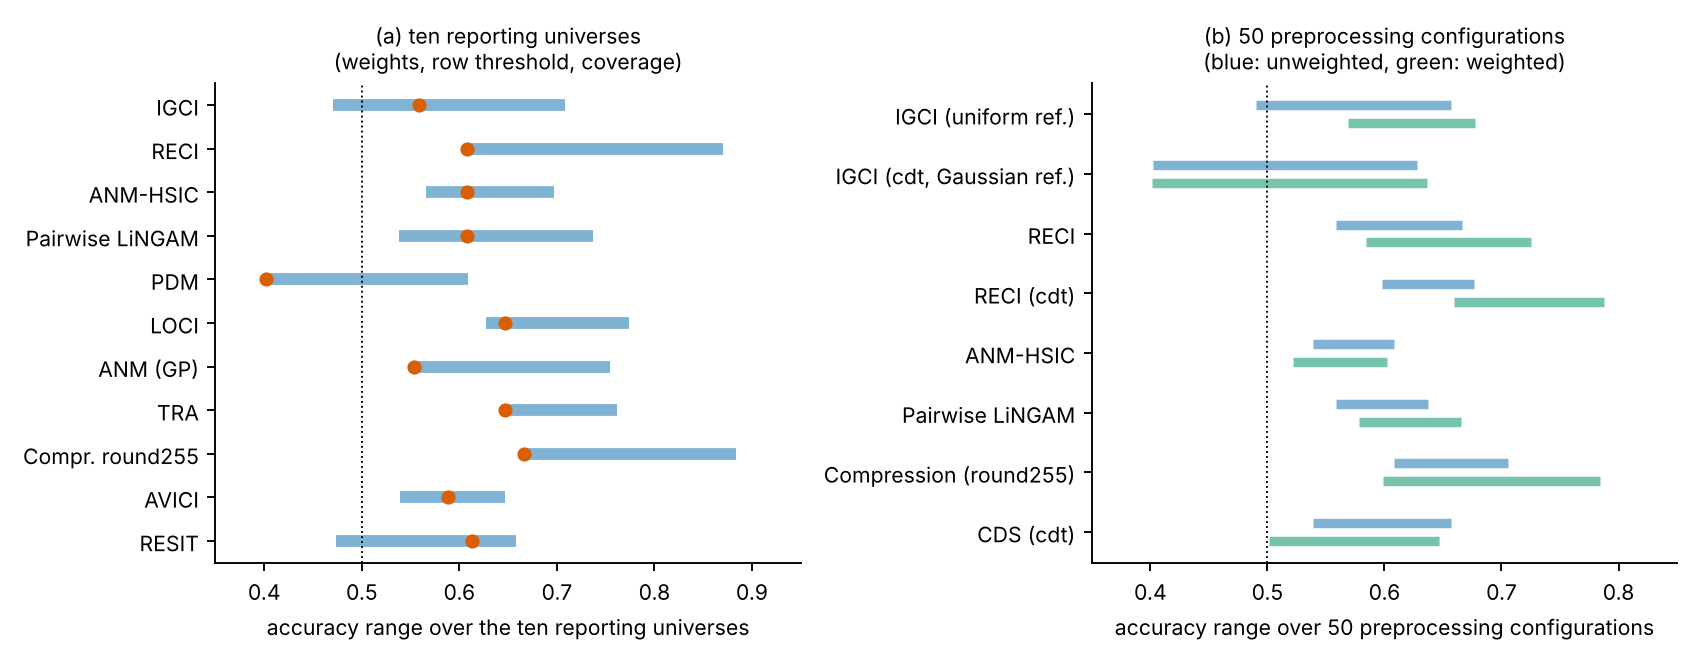
\includegraphics[width=\linewidth]{figs/fig4_freedom.png}
\caption{The range of each rule's accuracy on T\"ubingen (a) over ten defensible reporting universes (dot: accuracy on all pairs, unweighted) and (b) over $50$ preprocessing configurations (number of rows, dequantisation, seed).}
\label{fig:freedom}
\end{figure}

Single choices can be large. The official weights move RECI from $60.8\%$ to $70.9\%$, round255 compression from $66.7\%$ to $74.7\%$, and the floor256 variant from $60.8\%$ to $68.0\%$, while LOCI goes from $64.7\%$ to $63.9\%$. The quantisation convention of the compression rule (Section~\ref{sec:audit}) moves the weighted accuracy between $68.8$ and $74.7\%$.

Selecting among random subsets of $50$ pairs inflates the expected best accuracy of every rule by seven to eight points after ten tries without changing the order of the rules (Appendix~\ref{app:subsets}).

\subsection{A protocol multiverse on T\"ubingen}\label{sec:protocol_multiverse}

Section~\ref{sec:multi} varied how a result is reported. Here we vary how the data are prepared, for the same rule and the same pairs (experiment 61): the number of rows ($250$, $500$, $1000$, $2000$ or all, drawn at random), whether tied values are dequantised, and the seed (which changes the subsample and the rule's own randomness): $50$ configurations. Appendix Table~\ref{tab:protocol} gives the range of each rule's accuracy and the range of the marginal means of each factor.



The same rule on the same pairs moves by $7$ to $22$ points unweighted and $8$ to $23$ points weighted: IGCI with a uniform reference from $49.0$ to $65.7\%$, with cdt's Gaussian reference from $40.2$ to $62.7\%$ (the dequantisation alone: $52.4\%$ against $63.8\%$ on average for ours, so on raw T\"ubingen arrays IGCI is better than RECI, and with dequantisation worse), RECI weighted from $58.4$ to $72.5\%$, round255 compression weighted from $59.9$ to $78.4\%$, CDS unweighted from $53.9$ to $65.7\%$. The number of rows matters little on average (a few points) but through the random subsample the seed alone moves RECI, LiNGAM and ANM-HSIC by two to three points. The range of a single rule across protocol choices is as large as the range between the twelve rules of Appendix Table~\ref{tab:collections2} on T\"ubingen ($40$ to $67\%$, or $55$ to $67\%$ without the classifier below chance), and larger than the $2$ to $5$ points by which methods are usually separated. A comparison between two rules is therefore informative only under one identical protocol, run with the same preprocessing and several seeds; a comparison against a number quoted from a paper is not.
